\documentclass[a4paper]{report}

\usepackage{amsmath}
\usepackage{amssymb}
\usepackage{amsthm}
\usepackage{tcolorbox} % for colorboxes
\usepackage{minted} % for code highlighting
\usepackage{xcolor} % for own colors
\usepackage[margin=3.8cm]{geometry} % custom page margin
\usepackage[english]{babel}
\usepackage{graphicx} % using images

\graphicspath{ {./assets/} } % setting the path for images

% LimeGreen!40
% blue!20
% purple!20
% orange!40
% Emerald!40

\definecolor{dcGrayLight}{gray}{0.95}
\definecolor{dcOrange}{RGB}{255, 128, 0}
\definecolor{dcGreen}{RGB}{117, 225, 102}
\definecolor{dcBlue}{RGB}{99, 203, 255}
\definecolor{dcRed}{RGB}{255,88,88}
\definecolor{dcWhite}{RGB}{255, 255, 255}
\colorlet{dcRedLight}{red!5!white}

\newtcolorbox{definition}[1][]{
    colframe=dcBlue,
    colback = white,
    coltitle = black,
    title = \textbf{Definition}
}

\newtcolorbox{lemma}[1][]{
    colframe=dcGreen,
    colback = white,
    coltitle = black,
    title = \textbf{Lemma}
}

\newtcolorbox{satz}[1][]{
    colframe=dcRed,
    colback = white,
    coltitle = black,
    title = \textbf{#1}
}

\setlength{\parindent}{0in} % remove indentation for paragraphs

\title{Digital Design and Computer Architecture}
\author{Danny Camenisch (dcamenisch)}

\begin{document}
\maketitle
\tableofcontents


% --------------------------
%   Templates and Examples
% --------------------------

\chapter{Template}
\section{tcolorbox}

\begin{definition}
    Definition...
\end{definition}

\begin{lemma}
    Lemma...
\end{lemma}

\begin{satz}[Satz von Danny]
    Satz...
\end{satz}

\begin{tcolorbox}[colback=dcWhite,colframe=dcOrange,title=\textbf{My Heading}]
    This is a \textbf{tcolorbox}.
\tcblower
    Here, you see the lower part of the box.
\tcbsubtitle{subtitle}
\end{tcolorbox}

\section{minted}

\begin{minted}[frame=lines, framesep=2mm, bgcolor=dcGrayLight, linenos]{java}
    // Hello.java
    import javax.swing.JApplet;
    import java.awt.Graphics;
    
    public class Hello extends JApplet {
        public void paintComponent(Graphics g) {
            g.drawString("Hello, world!", 65, 95);
        }    
    }
\end{minted}


% minted can also import from file like this:
% \inputminted{java}{main.java}

% Including images
%\begin{figure}[h]
%    \centering
%    \includegraphics[width=\textwidth]{block_graph.png}
%    \caption{Beispiel eines Block-Graphen (links) und der }
%\end{figure}
%

% --------------------------
%   1. Introduction
% --------------------------
\chapter{Introduction}
\section{Description}

The class provides a first introduction to the design of digital circuits and 
computer architecture. It covers technical foundations of how a computing platform 
is designed from the bottom up. It introduces various execution paradigms, hardware 
description languages, and principles in digital design and computer architecture. 
The focus is on fundamental techniques employed in the design of modern microprocessors 
and their hardware/software interface.
\bigskip

\begin{satz}[Overview]
    This class provides a first approach to Computer Architecture. The students learn the
    design of digital circuits in order to:
    \begin{itemize}
        \item understand the basics
        \item understand the principles of design
        \item understand the precedents in computer architecture
    \end{itemize}
\tcblower
    Based on such understanding, the students are expected to:
    \begin{itemize}
        \item learn how a modern computer works underneath, from the bottom up
        \item evaluate tradeoffs of different designs and ideas
        \item implement a principled design (a simple microprocessor) 
        \item learn to systematically debug increasingly complex systems
        \item hopefully be prepared to develop novel, out-of-the-box designs
    \end{itemize}
    
\end{satz}
\bigskip

The focus is on basics, principles, precedents, and how to use them to 
create/implement good designs.

% --------------------------
%   2. Basics
% --------------------------

\chapter{Basics}

\section{Definitions}

In this script we will use the terms '1', TRUE and HIGH synonymously. Similarly, we will use '0', FALSE and LOW. Further 
we will use two's complement for signed binary numbers.

\section{Design and Choices}

Microprocessors where and still are a fundamental building block for the technological progess in the past
three decades. Without them things like the Internet and cell phones would not exist. But for the
development of new chips performance is not always the main priority. While performance is important,
there is always a tradeoff between many different other aspects, including power consumption, temperature
price and size, only to mention some of them. \\

Systems like a microprocessor can get really complicated to understand on a low level. To get a better
understanding of such a system, it is necessary to use different techniques:
\begin{itemize}
    \item Abstraction: hiding details when they are not important
    \item Disciplin: intentionally restricting design choices so that you can work more productively at a higher level of abstraction
    \item Hierarchy, Modularity, Regularity: defining a clear structure dividing a system into well-defined modules and reusing them among multiple points
\end{itemize} 

Microarchitecture links the logic and architecture levels of abstraction. This will be the main focuse of this course.

\begin{figure}[h]
    \centering
    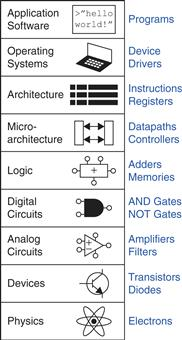
\includegraphics[width=3cm]{abstractionLevels.jpg}
    \caption{Levels of abstraction for a electronic computing system}
\end{figure}

\pagebreak

\section{Representing Numbers}

There are three commonly used systems to represent numbers. We normally use decimal numbers, but
in digital systems binary and hexadecimal numbers are more convienient. It is assumed that the reader
is familiary with using these number systems and knows how to performe simple operations in them. When
dealing with addition one has to be carefull to check for overflow of the carry bit.

\begin{satz}[Important Terms]
    \begin{itemize}
        \item \textbf{Bit}: A single 0 or 1
        \item \textbf{Byte}: A group of eight bits, can be represented by two hexadecimal digit
        \item \textbf{Nibble}: Half a byte, can be represented by one hexadecimal digit
        \item \textbf{Word}: Data chunks a microprocessor handels, today 64 or 32 bit
        \item \textbf{LSB}: least significant bit, right-most bit in a group of bits
        \item \textbf{MSB}: most significant bit, left-most bit in a group of bits
    \end{itemize}
\end{satz}

There are multiple ways to represent a negative number in the binary system. The two most common ones are
called sign/magnitude and two's complement. \\

\textbf{Sign/Magnitude}: We use the MSB as a sign bit, this causes the problems that addition will no longer work
and there exists both $+0$ and $-0$. This covers the range $[-2^{N-1}+1, 2^{N-1}-1]$. \\

\textbf{Two's Complement}: Same system as a unsigned binary number except the MSB has a weight of $-2^{N-1}$.
Here addition works fine and there is only one representation for $0$. The process of creating a negative number
consists of inverting all the bits of the number and adding $1$ to the LSB. This covers the range $[-2^{N-1}, 2^{N-1}-1]$.

\section{Logic Gates}

Logic Gates are simple digital circuits that take one or more binary inputs (denoted by letters from the beginning of the alphabet) and 
produce a binary output (commonly denoted Y). The most common logic gates are: \\

\begin{figure}[h]
    \centering
    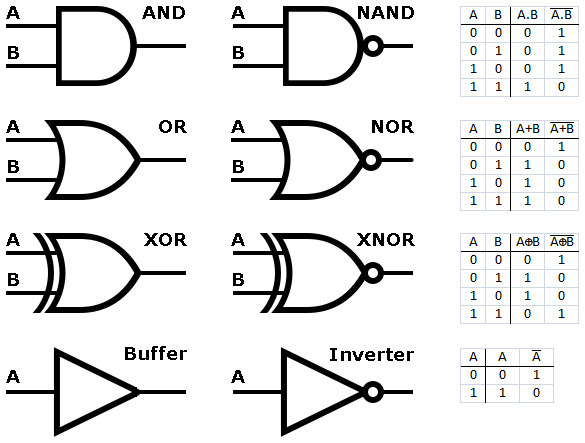
\includegraphics[width=9cm]{gates.png}
    \caption{Most important logic gates}
\end{figure}

Note that a N-input XOR produces a TRUE output when an odd number of inputs are TRUE. From a logical point of view, a buffer 
might seem useless. However, from the analog point of view, the buffer has multiple, desirable characteristics such as the 
ability to quickly send its output to many gates. The logic operations can be denoted as follows:

\begin{center}
    \begin{tabular}{ c  l }
        BUFFER & $Y = A$  \\ 
        NOT & $Y = \overline{A}$  \\ 
        AND & $Y = A \cdot B = AB = A \cap  B$  \\ 
        OR & $Y = A + B = A \cup B $  \\ 
        XOR & $Y = A \oplus B$  \\ 
        NAND & $Y = \overline{AB}$  \\   
        NOR & $Y = \overline{A + B}$ \\
        XNOR & $Y = \overline{A \oplus B}$
    \end{tabular}
\end{center}

There also exist logic gates with more than two inputs.

\section{Beneath the Abstraction}

\paragraph{Supply Voltage:} In reality, binary signals are represented with a voltage on a wire. The lowest
voltage in a system (0 V) is called the ground GND and the highest is denotes as $V_{DD}$ (between 1.2 and 3.3 V).

\paragraph{Noise:} Since in reality this signal is analog and could theoretically have every value between GND and $V_{DD}$ it could
be that we encounter noise. We can use a trick to filter such noise and get a clear signal. The noise margin
is the amount of noise we can add to a signal and it can still be correctly interpreted. In this example we look
at two simple logic gates, a driver and receiver. The noise margin is calculated $NM_L = V_{IL} - V_{OL}$, 
$NM_H = V_{OH} - V_{IH}$.

\begin{figure}[h]
    \centering
    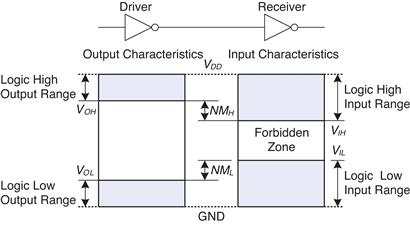
\includegraphics[width=9cm]{noise.jpg}
    \caption{Example}
\end{figure}

\paragraph{CMOS Transistors:} We skip the detailed explanation of how a transistor works and look at what it does.
A transistor can be viewed as a electrically controlled switch that turns ON or OFF when a voltage is applied to a
controll terminal. The most common transistors are MOS transistors (or MOSFET). There are two types nMOS and pMOS. \\

\begin{figure}[h]
    \centering
    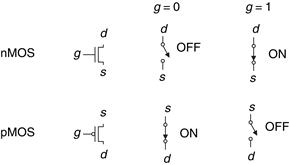
\includegraphics[width=9cm]{mosfet.jpg}
    \caption{MOS transistors}
\end{figure}

\paragraph{Logic Gates:} We can use transistor to build logic gates, as an example we will have a look at how a AND gate is
built. A AND gate consists of a NAND gate and a NOT gate, that are made up by transistors as can be seen in the figure.

\begin{figure}[h]
    \centering
    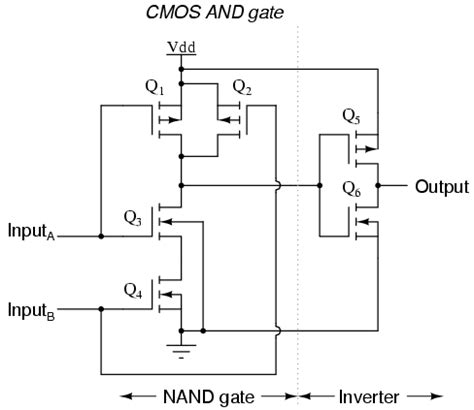
\includegraphics[width=8cm]{cmosAnd.jpeg}
    \caption{MOS transistors}
\end{figure}

\chapter{Combination Logic Design}

\section{Introduction}
A \textbf{circuit} is a network that processes distinct-value variables. It has:
\begin{itemize}
    \item one or more input terminals
    \item one or more output terminals
    \item a functional specification (expressed by a truth table)
    \item a timing specification
\end{itemize}
Digital circuits are classified as \textbf{sequential} or \textbf{combinational} (this chapter will discuss the later one). The difference
between these two is, that a combinational circuit combines the current input values to compute the output, whereas in a sequential circuit,
the output depends on the current input and on the previous input values. In another way, a combinational circuit is \textbf{memoryless} and 
a sequential circuit has \textbf{memory}. \\

Combination circuit therefore have to satisfie the following requirements:
\begin{itemize}
    \item every circuit (element) is itself combinational
    \item every wire (node) of the circuit is either designated as input or output
    \item the circuit contains no cyclic paths
\end{itemize}

\section{Boolean Algebra}

\begin{definition}
    \begin{itemize}
        \item \textbf{Complement} - The inverse of a variable, $\bar{A}$
        \item \textbf{Literal} - A variable in a equation
        \item \textbf{Product} - The AND of two or more literals
        \item \textbf{Minterm} - The product of all inputs (or their complement) of a function
        \item \textbf{Sum} - The OR of two or more literals
        \item \textbf{Maxterm} - The sum of all inverse of inputs (or their complement) of a function
        \item \textbf{Precedence} - The order of operations: NOT > AND > OR
        \item \textbf{Sum of product form (SOP)} - The sum of all minterms for which a function is true
        \item \textbf{Product of sum form (POS)} - The product of all maxterms for which a function is false
        \item \textbf{Prime implication} - An implicant that cannot be combined with other implicants to for a new implicant with fewer literals
    \end{itemize}
\end{definition}

\subsection{Axioms and Theorems}

\begin{figure}[h]
    \centering
    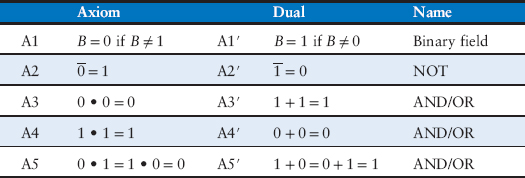
\includegraphics[width=10cm]{axiom.jpg}
    \caption{Axioms}
\end{figure}

\begin{figure}[h]
    \centering
    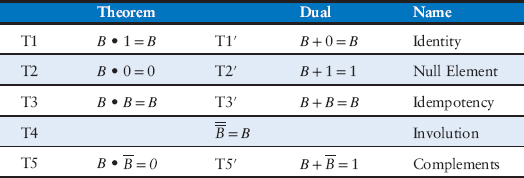
\includegraphics[width=10cm]{theorem.jpg}
    \caption{Theorems}
\end{figure}

\begin{figure}[h]
    \centering
    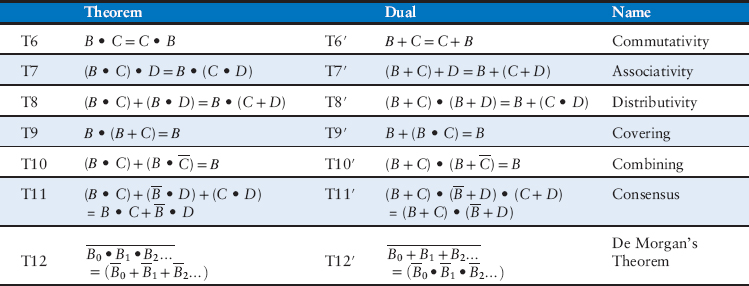
\includegraphics[width=10cm]{theorem multiple.jpg}
    \caption{Theorems for multiple variables}
\end{figure}

\pagebreak
We can use these helpful theorems to reduce boolean equations into prime implicants.

\section{From Logic to Gates}
When drawing a \textbf{schemantic} we generally follow these rules:
\begin{itemize}
    \item Inputs are on the left / top side
    \item Ouputs are on the right / bottom side
    \item Gates should flow from left to right
    \item Straight wires are better
    \item Wires always connect at a T Junction
    \item Wires crossing without a dot make no connection
\end{itemize}
To draw such a schemantic it can be usefull to first draw a truth table. In a truth table a X marks a don't care.

\section{Multilevel Combinational Logic}
In this section we will shortly mention bubble pushing as a helpful way to redraw combinational circuits so that bubbles cancel
out and the function can be more easily determined. (More details can be found in the book)

\section{Illegal and Floating Values}
The symbol X indicates that the circuit node has an \textbf{unknown} or \textbf{illegal} value, this commonly happens if a node
is being driven both by a 0 and a 1 at the same time. This situation is also called \textbf{contention}. Be carefull to not mistake this
X with a don't care in truth tables. \\

The symbol Z denotes that a node is being driven neither by HIGH nor LOW. The node is said to be \textbf{floating, heigh impedance} or \textbf{high Z}.
In reality, a floating node might be 0 or 1 or something in between.

\section{Karnaugh Maps}
Karnaugh Maps are a usefull graphical method for simplifying Boolean equations. They work well for equations with up to four
variables. 

\begin{figure}[h]
    \centering
    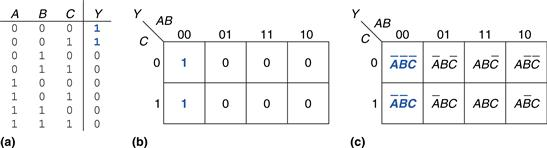
\includegraphics[width=13cm]{karnaugh.jpg}
    \caption{A Karnaugh Maps}
\end{figure}

Note that the AB combinations are in Gray code.

\begin{figure}[h]
    \centering
    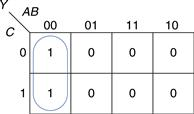
\includegraphics[width=6cm]{karnaugh2.jpg}
    \caption{A Karnaugh Maps}
\end{figure}

We use the following rules to minimize a expression using a K-map:
\begin{itemize}
    \item Us the fewest circles necessary to cover all 1's
    \item A circle can only contain 1's
    \item Each circle must span a rectangular block that is a power of 2 in each direction
    \item Each circle should be as large as possible
    \item A circle may wrap around the edge of the K-map
    \item A 1 in a K-map may be circled multiple times
\end{itemize}

\section{Combinational Building Blocks}
Combinational Logic is often grouped into larger building blocks to build more complex systems. This is an application fo the
principle of abstraction. Some of these building blocks are full adders, priority circuits and seven-segment display decoders.
In this section we will look at another two building blocks.

\subsection{Multiplexer (mux)}

Multiplexers (short mux) are among the most commonly used combinational circuits. They choose an output among 
several possible inputs based on the value of a select signal. A 2:1 mux chooses between 2 different input signals.

\begin{figure}[h]
    \centering
    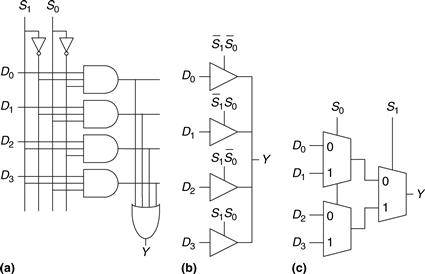
\includegraphics[width=11cm]{mux.jpg}
    \caption{4:1 mux implementations}
\end{figure}

\subsection{Decoders}
A decoder has $n$ inputs and $2^n$ outputs. It asserts exactly one of its outputs depending on the input combination.
The output of a decoder are called \textbf{one-hot}, because exactly one of them is hot at a given time.

\begin{figure}[h]
    \centering
    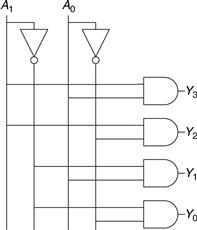
\includegraphics[width=6cm]{decoder.jpg}
    \caption{2:4 decoder}
\end{figure}

\pagebreak
\section{Timing}
An output takes time to change in response to a change of input. We can draw a \textbf{timing diagram} to visialize the
transient response of a combinational circuit. The transition from LOW to HIGH is called the \textbf{rising edge} and from HIGH
to LOW it's called the \textbf{falling edge}. 

\begin{figure}[h]
    \centering
    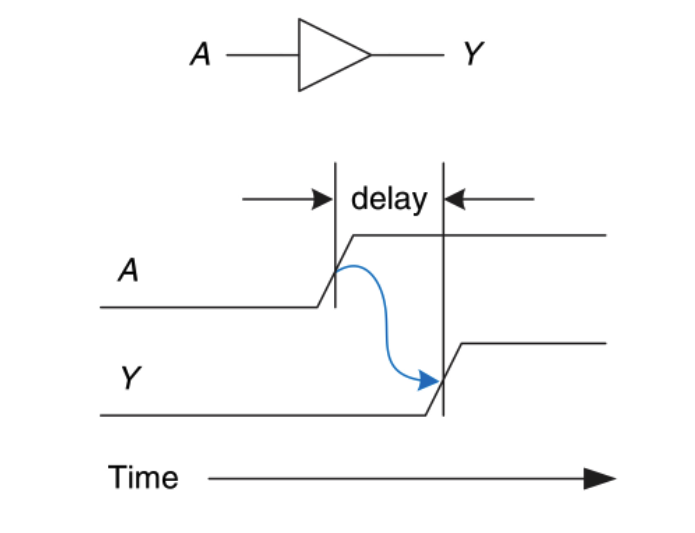
\includegraphics[width=10cm]{timing.png}
    \caption{timing diagram of a buffer}
\end{figure}

Combinational logic is characterized by its \textbf{propagation delay $t_{pd}$}, the maximum time from when a input changes
until the output reaches their final state, and the \textbf{contamination delay $t_{cd}$}, the minimum time from an input 
change until the output starts changing. \\

Since $t_{pd}$ and $t_{cd}$ are determined by signal paths in a combinational circuit, we introduce the following two 
definitions: 
\begin{itemize}
    \item \textbf{Critical path} - The longest and therefore slowest path in a circuit
    \item \textbf{Short path} - The shortest and therefore fastest path through a circuit
\end{itemize}
We can now calculate the $t_{pd}$ by adding up the propagation time for each element along the critical path, and similarly calculate 
the $t_{cp}$ by adding all propagation times along the short path.

\end{document}
